\documentclass[12pt, letterpaper, titlepage]{article}

\usepackage{amsmath}
\usepackage{booktabs}
\usepackage{amsthm}
\usepackage{graphicx}
\usepackage[margin=1in]{geometry}
\usepackage{hyperref}
\usepackage{cleveref}
\hypersetup{colorlinks = true, linkcolor = blue, citecolor=blue, urlcolor = blue}
\usepackage{natbib}
\usepackage{float}
\usepackage{setspace}
\usepackage{pdfpages}
\usepackage[pagewise]{lineno}
\usepackage{mwe}
%\linenumbers*[1]
% %% patches to make lineno work better with amsmath
\newcommand*\patchAmsMathEnvironmentForLineno[1]{%
 \expandafter\let\csname old#1\expandafter\endcsname\csname #1\endcsname
 \expandafter\let\csname oldend#1\expandafter\endcsname\csname end#1\endcsname
 \renewenvironment{#1}%
 {\linenomath\csname old#1\endcsname}%
 {\csname oldend#1\endcsname\endlinenomath}}%
\newcommand*\patchBothAmsMathEnvironmentsForLineno[1]{%
 \patchAmsMathEnvironmentForLineno{#1}%
 \patchAmsMathEnvironmentForLineno{#1*}}%

\AtBeginDocument{%
 \patchBothAmsMathEnvironmentsForLineno{equation}%
 \patchBothAmsMathEnvironmentsForLineno{align}%
 \patchBothAmsMathEnvironmentsForLineno{flalign}%
 \patchBothAmsMathEnvironmentsForLineno{alignat}%
 \patchBothAmsMathEnvironmentsForLineno{gather}%
 \patchBothAmsMathEnvironmentsForLineno{multline}%
}

% control floats
\renewcommand\floatpagefraction{.9}
\renewcommand\topfraction{.9}
\renewcommand\bottomfraction{.9}
\renewcommand\textfraction{.1}
\setcounter{totalnumber}{50}
\setcounter{topnumber}{50}
\setcounter{bottomnumber}{50}

\newcommand{\jy}[1]{\textcolor{blue}{JY: #1}}
\newcommand{\eds}[1]{\textcolor{red}{EDS: (#1)}}


\title{Was Devon Allen Unjustly Disqualified at the 2022 World Track and Field Championships?} 

\author{Owen Fiore\\
%   \href{mailto:owen.fiore@uconn.edu}
% {\nolinkurl{owen.fiore@uconn.edu}}\\
  Elizabeth Schifano\\
  Jun Yan\\[1ex]
  Department of Statistics, University of Connecticut\\
}
\date{}

\begin{document}
\maketitle

\doublespace

\begin{abstract}
  At the 2022 World Track Championships in Eugene Oregon, Devon Allen was disqualified in the
  Men's 110 meter hurdle final after registering a reaction time of 0.099 seconds, 0.001 
  seconds faster than what is allowed.  Following the games, bloggers on the running website 
  LetsRun scrutinized the results and performed non-statistical analysis of the data \citep{Johnson}
  They found that the reaction time data from the 2022 World Track Championships seemed to be faster 
  compared to the other datasets they looked at, but did not perform any meaningful statistical 
  analysis of the data.  Devon Allen had previously ran the third fastest time in history when 
  he ran 12.84 earlier in 2022 and was considered to be one of the favorites to win \citep{Preview}.  His 
  disqualification thus prompted questions into whether the timing equipment used at the World
  Track Championships was accurate and whether or not Allen actually reacted as fast as the 
  timing equipment stated he did.

%\bigskip
\noindent\sc{Keywords}:
Devon Allen, Reaction Time, Seiko, 2022 World Track and Field Championships 

\end{abstract}



\section{Introduction}
\label{sec:intro}

Other scholarly papers have discussed track and field reaction times but not in the
context of whether the minimum reaction time barrier is too low or whether or not timing
systems were accurate.  Outside of the blog posts from LetsRun.com, there have not been
any published papers regarding Devon Allen's disqualification in particular.  This is not
neccessarily suprising given that the World Track and Field Championships occurred only 
four months ago.

The contribution of this paper is to question whether or not Seiko's timing data
was accurate and thus if Devon Allen was disqualified more so because of faulty
equipment rather than reacting illegally fast.  There is little at this point
that could be done to rectify any potential mis-qualification other than to try
to prevent it from happening again.  THis matter needs to be addressed because Devon Allen's 
disqulification could be a problem that could continue to re-appear.  If athletes
are reacting fast enough that the timing system thinks that they are reacting
illegally fast, then World Athletics needs to address this and possibly change
the minimum reaction time allowed.  Currently the barrier is 0.10 seconds, any time
faster than this would result in a disqualification in the athlete who reacted too
quickly and the race is restarted \citep{Seiko-Timing}.  Since 2011, any athletes who false 
start are not given a second chance, they are removed from competition \citep{False-Start}.  
This can have massive implications as events like the Outdoor World Track and Field Championship 
only occur typically once every two years.  It is an opportunity for athletes to earn endorsement
deals and prove to sponsors such as Nike and Adidas that
they deserve a contract.  Thus the significance of a disqualification, especially in the finals 
of a major event such as the World Track and Field Championships, are very
consequential.  

\section{Background}
\label{sec:Background}
Since 1985 Seiko Holding Corporations has served every World Athletics Championship
as the official timer \citep{Seiko}.  Since 1985, the technology and the ability
to accurately predict measurements: long jump distances, false starts, total time,
reaction time, etc. have all dramatically improved.  Seiko did not start tracking
reaction time as an official measurement until 1999 in the men's and women's 100 meter
hurdles.  Seiko regularly updates their equipment so that they provide cutting edge
technology to the World Track and Field Championships, the highest stakes in the world
of running outside of the Olympics.

%Citation needed in this section
Seiko's technology for detecting reaction times relies on the pressure that athletes
exert on the plate when they push off.  Their systems measure the time differential
between when the "gun" goes off to start the race and when the pressure changes 
\citep{Seiko}  If an athlete has a reaction time under 0.10 seconds, it is deemed a 
false start as it is considered that no athlete can react so quickly \citep{Seiko-Timing}.  
Thus, a reaction time of for example 0.05, suggests that the athlete predicted the gun and it
was luck that caused their abnormally high time.  At the World Championship level,
World Athletics and Seiko want to remove that element of luck and thus impose the 0.1
second barrier.

In 2013, Seiko upgraded their timing equipment for sprinting events (100 meter hurdles
falls under this catergory) \citep{WorldAthletics_2013}.  Since 1999, the highest reaction 
times in the men's 100 meter hurdle were recorded in 2013.  That is not to say that the higher 
times were caused by Seiko's equipment, but the two may be related.  It is worth noting that prior
to 2022, Seiko again upgraded its technology but for its jump management system.

Something that is extremely important to note in the Data is the inconsistency of World Athletics 
in terms of how they penalize false starts.  From 2007-2009, the IAAF (the former name for World 
Athletics, and the governing body for the World Track and Field Champions) instituted a rule change
that allowed one warning false start before a sprinter was disqualified \citep{False-Start}  This 
essentially gave sprinters a second chance and reduced the penalty for a false start.  There were 
18 male and 7 female false starts at the 2007 World Championships, 18 male and 7 female starts at 
the 2009 World Championships. Starting in 2011, the rule was scrapped, and the old policy which 
automatically disqualifies runners who false start was reinsituted.  The effect? At the 2011 World
Championship there were 6 male disqualifications and 4 female disqualifications \citep{False-Start}. 
By returning to the harsher policy and cracking down on false starts, World Athletics had reduced the
number of false starts by two thirds. This was desirable for World Athletics as false starts can 
make already long track meets more tedious, both for athletes and viewers watching the 
television broadcast.\citep{Pilianidis}

\section{Data}
\label{sec:Data}
Data was copied from the World Athletics website and pasted into an excel
spreadsheet. The data covers the men's 110 meter hurdles and the women's 100
meter hurdles from 1999 to 2022.  The variable of prediction interest is reaction
time, and the predicting variables are year, stage of competition (heats, 
semifinal, final), total time, and gender.  The data can be found in the appendix:.  
Factors such as name, country, and identification number were
not considered important for the purposes of this research besides the times for
Devon Allen and the other United States athletes mentioned above.  The variable "Stage"
refers to whether the observation occurred during the "heats" (Preliminary round) which
is denoted by "H" in the data, "S" for "semifinals" (Of which there are either 2 or 3 
heats each year), and "F" for finals. The variable "Gender" has levels "M" and "F" 
which stand for "male" and "female" respectively.  The variable "Batch" takes a 
numerical value and every heat of every round from 1999 to 2022 was assigned it's
own number.  This was added because of suspected issues that reaction time may be
correlated with other runners reacting quickly (one runner reacting quickly may
result in other runners reacting quickly).  There is no statistical signficance to
how the batches were labeled, they were ordered chronologically by meet but
reverse chronologically by year (Batch 1 is a preliminary Heat of 2022 and Batch
111 corresponds to the 1999 finals). The data that looked at in the paper
is best visualized using a scatterplot and box plot. Figure~\ref{fig:DataBoxPlot}
below shows the box plot data.
\begin{figure}[h]
  \centering 
  \includegraphics[scale = 0.5]{DataBoxPlot}
  \label{fig:DataBoxPlot}
\end{figure}

\begin{figure}[h]
  \centering 
  \includegraphics[scale = 0.5]{DataScatterPlot}
  \label{fig:DataScatterPlot}
\end{figure}



One of the most interesting things found was that the reaction times from the USA
athletes in the World Championship 110 meter hurdles, was that they were significantly
faster than at the USA Track Championships.  From June 23-26 2022, USA held it's Track
and Field Championship to decide who to send to the World Championships at Hayward 
Field, the exact same venue as used for the World Track and Field Championship a month 
later.  Thus, a baseline is able to be established for the four USA athletes who 
competed in at least one round of both events: Trey Cunningham, Daniel Roberts, 
Grant Holloway, and Devon Allen. Every athlete reacted faster in all of the World 
Track and Field Championship races compared to the USA Track and Field 
Championship races. Devon Allen raced three times at the USA Track and
Field Championship and three times at the World Track and Field  Championship. 
His reaction times were significantly faster in the World Track and
Field Championship compared to the USA Track and Field Championship as were his
teamates.  This comparison suggests that the timing system used between the two
meets may have been meaningfully different to the point where Devon Allen was
disqualified more because of faulty equipment rather than because he reacted
too quickly.  This table below highlights the difference in reaction times for
Devon Allen, Trey Cunningham, Grant Holloway, and Daniel Roberts. "USA" denotes
the USA Track and Field Championships, "World" denotes the World Track and Field
Championships, "N/A" was used for any athlete that did not compete and thus
did not register a reaction time.  All numbers listed in the table are the reaction
time for the respective athletes in seconds. 

\begin{center}
  \begin{tabular}{||c | c c c | c c c||} 
   \hline
   Athlete & USA H & USA S & USA F & World H & World S & World F \\ [0.5ex] 
   \hline\hline
   Devon Allen & 0.201 & 0.153 & 0.160 & 0.123 & 0.101 & 0.099 \\ 
   \hline
   Trey Cunningham & 0.186 & 0.185 & 0.182 & 0.115 & 0.120 & 0.109 \\
   \hline
   Grant Holloway & 0.192 & 0.190 & N/A & 0.147 & 0.128 & 0.124 \\
   \hline
   Daniel Roberts & 0.181 & 0.200 & 0.183 & 0.179 & N/A & N/A \\ [0.5ex]
   \hline
  \end{tabular}
  \end{center}


\section{Methods}
\label{sec:methods}

The main statistical model used in the paper is a gamma mixed effects model, which is
in the family of Generalized Linear Mixed Model (GLMM). The GLMM comes from the R package 
lme4, which hosts a variety of GLMM functions \citep{Rpkg:lme4}.  A GLMM is a type of model
that supports inputs that are from different distributions.  The model that we use is for the
Gamma distribution for the fixed effects part of the model and a random effects part.  In
the model used in the paper, the fixed effect comes in the form of an intercept, and then
either a year effect, batch effect, or both are used.  Initially a linear mixed effects
model was attempted to be implemented, but due to a right hand skew in the reaction times, 
a gamma distribution seemed better equipped to model the data (The rightskew is not 
particularly suprising as it is not possible to register a reaction time below 0.0 
seconds, resulting in a lower bound but no upper bound for outliers). In the code, the 
link parameter under Gamma() was changed to be "log" as logarithmic functions are better 
equipped to deal with high outliers.  The graph below shows the skewed outliers: ~\ref{fig:Skew}.
\begin{figure}[h]
  \centering 
  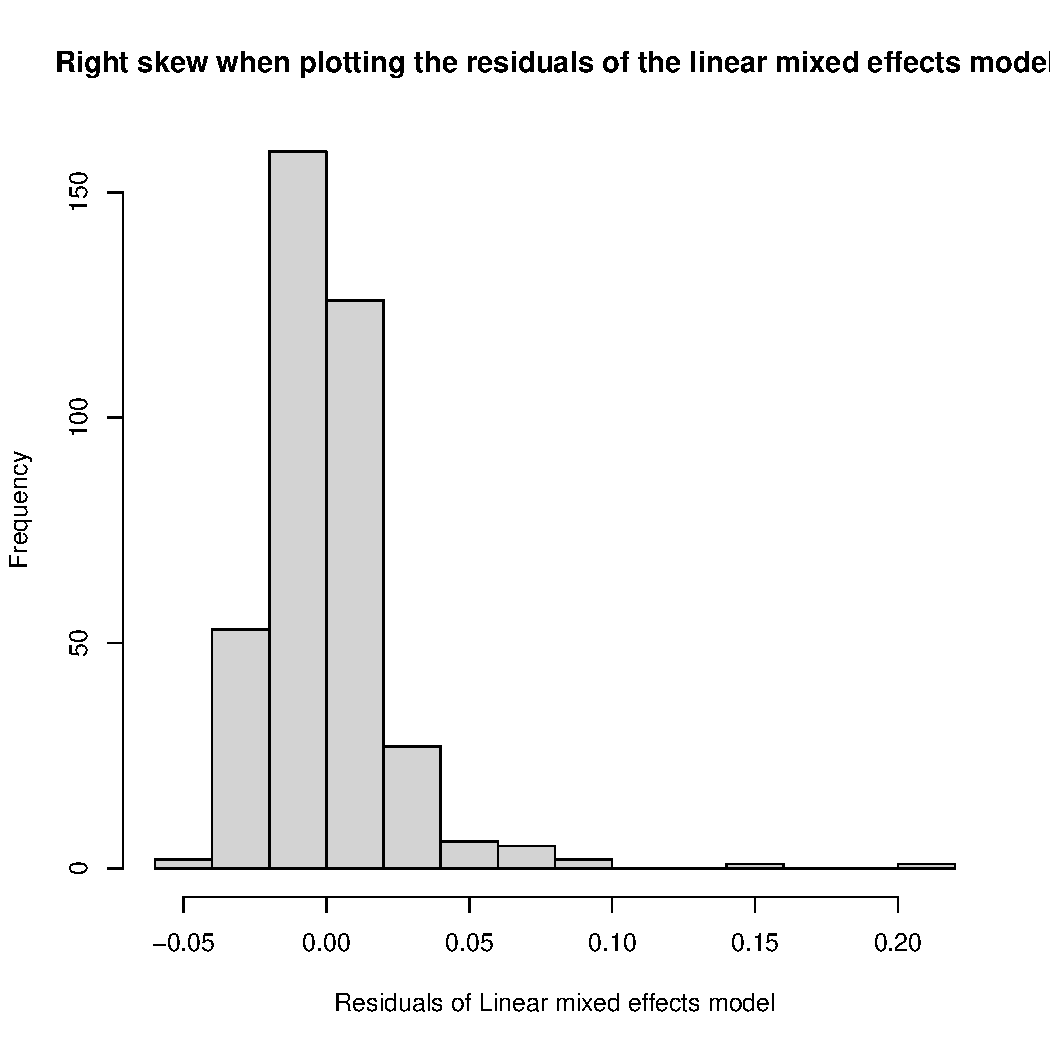
\includegraphics[scale = 0.6]{Skew}
  \label{fig:Skew}
\end{figure}


Once the Gamma mixed effects model was chosen, it needed to be decided which combination
of effects to use.  It was possible to include a year effect, a batch effect, or a year
and batch effect.  Density plots were created that simulated the probability of a mean
density less than 0.1, which is the current threshold for a reaction time
disqualification.  The density plots are shown below.

\begin{figure}[h]
  \centering
  \begin{minipage}{0.45\textwidth}
      \centering
      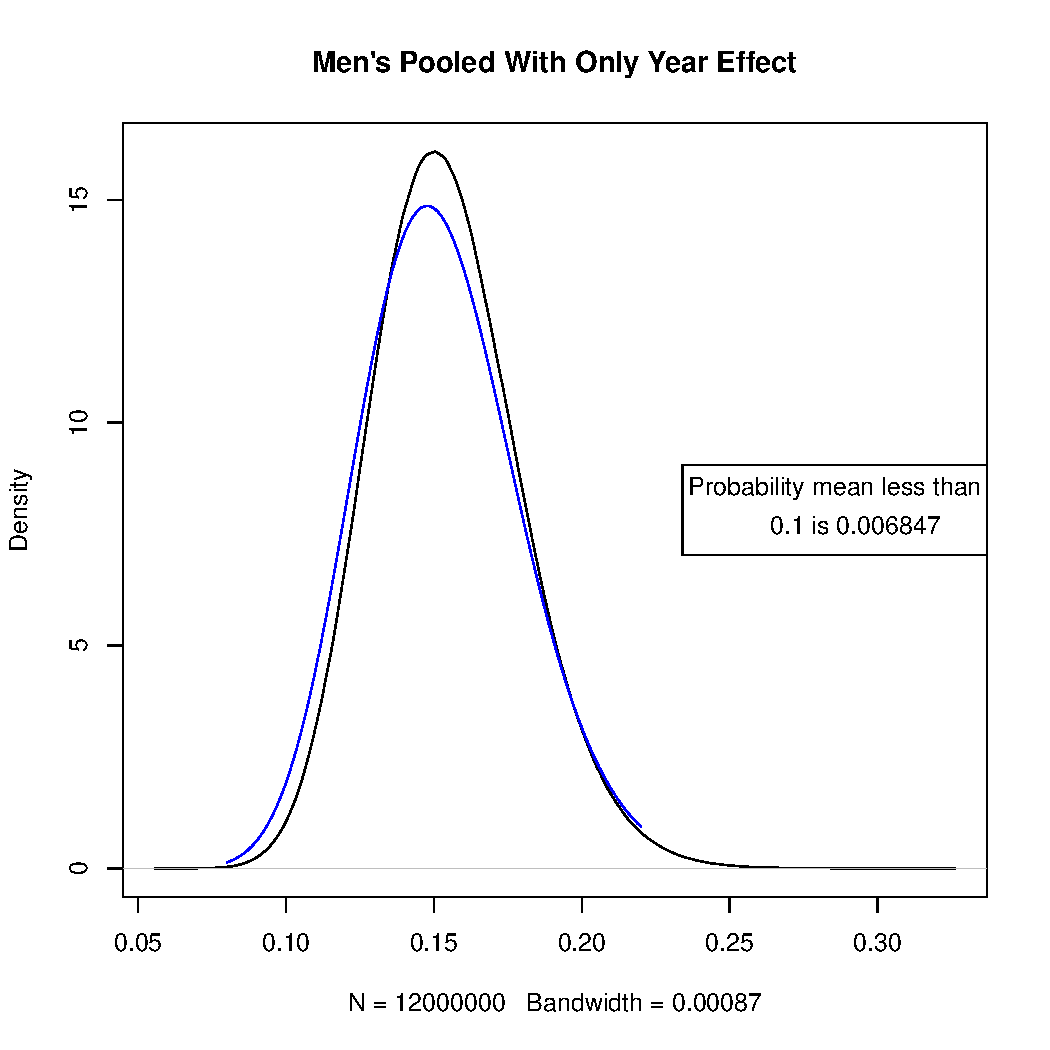
\includegraphics[width=0.9\textwidth]{Men_Density_Year} % first figure itself
      \caption{Density plot using pooled men's data and the year effect}
  \end{minipage}\hfill
  \begin{minipage}{0.45\textwidth}
      \centering
      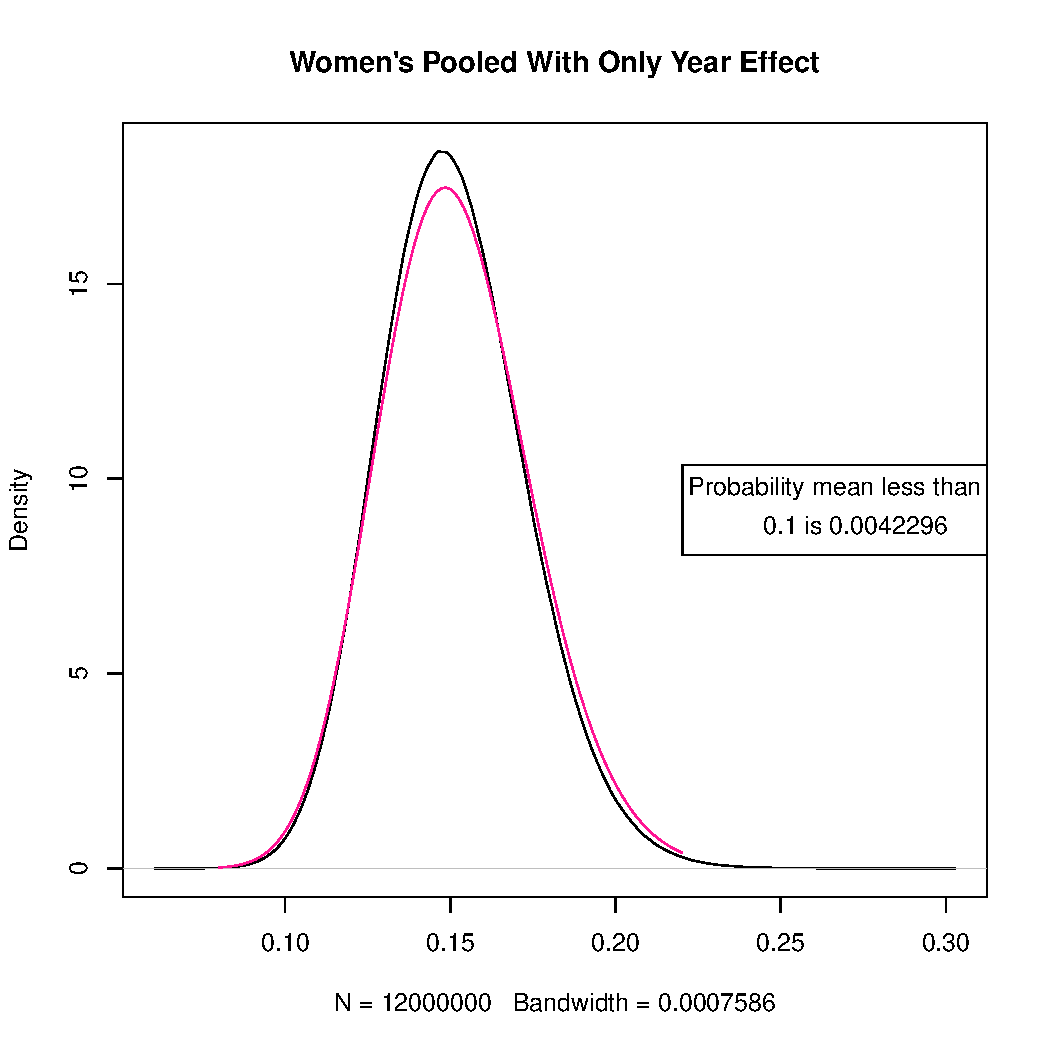
\includegraphics[width=0.9\textwidth]{Women_Density_Year} % second figure itself
      \caption{Density plot using pooled women's data and the year effect}
  \end{minipage}
\end{figure}

\begin{figure}[h]
  \centering
  \begin{minipage}{0.45\textwidth}
      \centering
      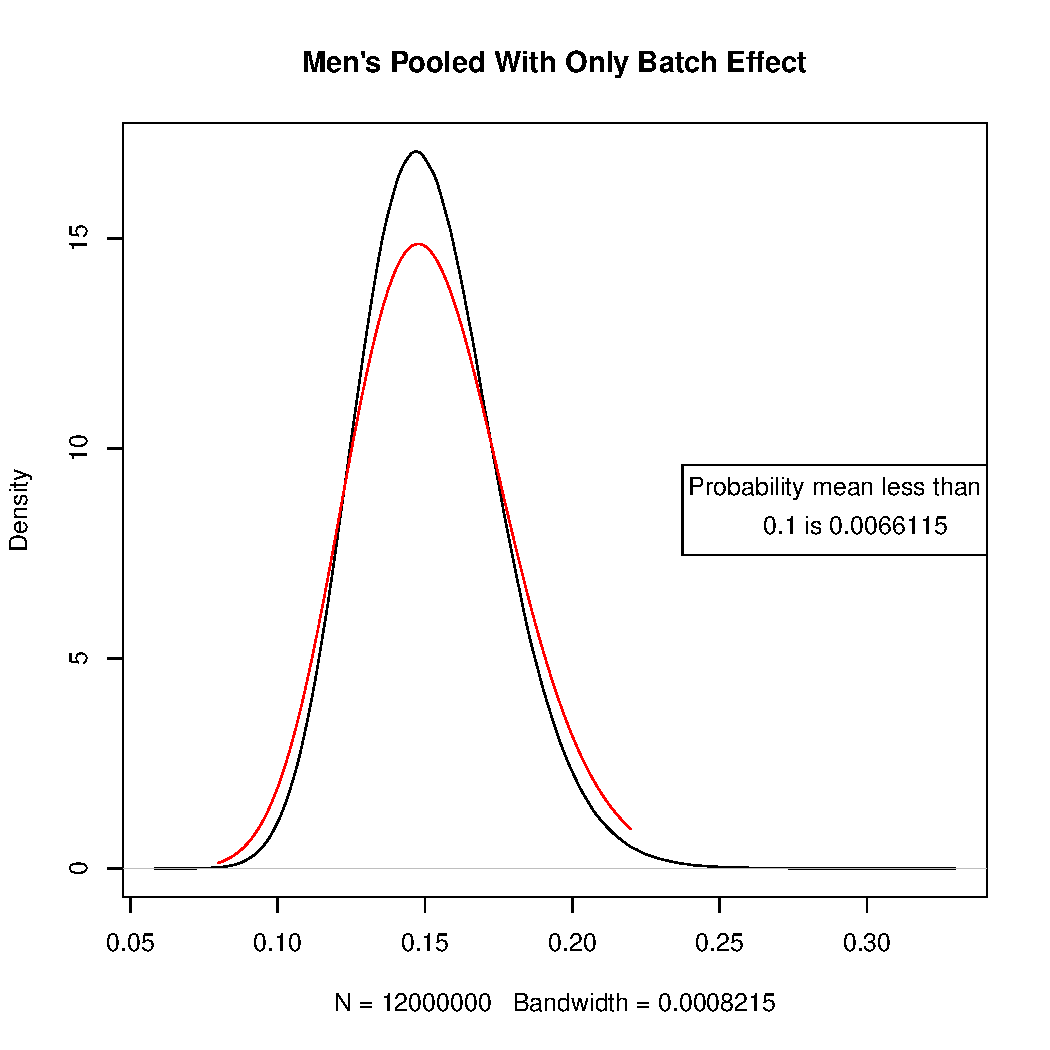
\includegraphics[width=0.9\textwidth]{Men_Density_Batch} % first figure itself
      \caption{Density plot using pooled men's data and the batch effect}
  \end{minipage}\hfill
  \begin{minipage}{0.45\textwidth}
      \centering
      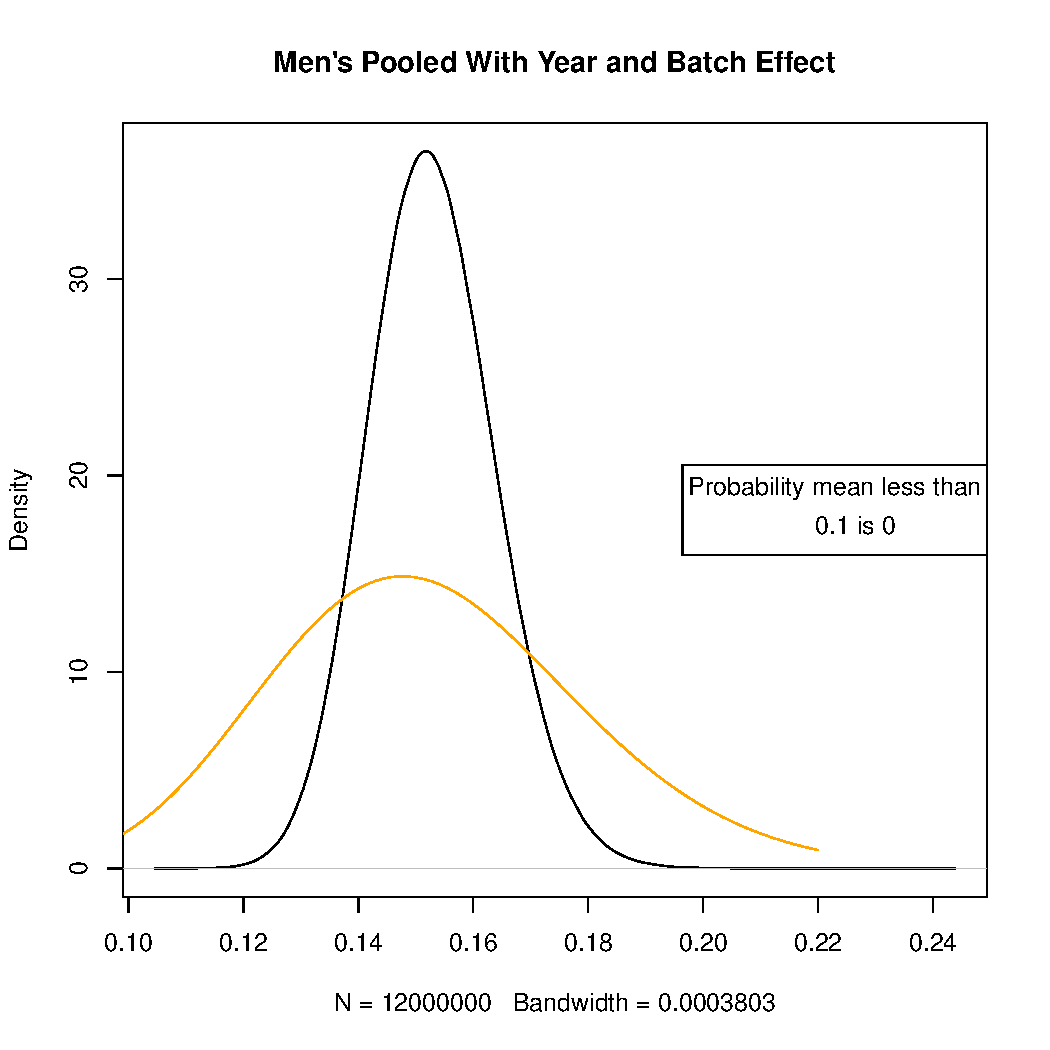
\includegraphics[width=0.9\textwidth]{Men_Density_Both} % second figure itself
      \caption{Density plot using pooled men's data and both year and batch effect}
  \end{minipage}
\end{figure}


There are several different data sets that could be used and explored in determining 
whether or not Devon Allen was unjustly disqualified.  One of the best examples of this
is the women's 100 meter hurdles. Although the distance of the race is 10 meters shorter
than the men's race, the reaction time data is still important and can be used to
essentially double the data size.  However, one of the largest issues with this is that on average, men are able to react quicker than women.  A study from the 2008 Beijing Olympics found that the p value of comparing the mean fastest reaction time between men and women was below 0.001 and the differnce is in part because of the greater force threshold men are able to exert on the starting blocks \citep{Lipps}. The data from including both men and women could follow a bimodal distribution which would be difficult to model and not helpful for determining if Devon Allen's reaction time was the result of a faulty system or if it is an argument
for changing the 0.10 second minimum barrier that currently exists.  Thus it was decided
to look at men's and women's data separately.  Another decision that was made was to look
at the data from the semifinals and finals together but from the heats or preliminary rounds.  The reason for this was because it was reasoned that in the finals athletes may
be a little more anxious, more "jumpy" and that under stress and they would react faster.
Additionally, exceptionally strong atheletes may not race as hard in the early heats in
order to reduce the risk for injury and to save themselves for the later stages of
competition that matter more. While the preliminary rounds also provide a bulk of the total observations, they are not as relevant to Allen's disqualification, which occured during the finals.  Thus, the decision was made to look at data from the men's semifinals
and finals in a "pooled" data set.
%%%Include picture 



\section{Conclusion}
\label{sec:conclusion}
It is worth noting that in the semi-finals of the World Track and
Field Championships; Allen's reaction time was 0.101 which is only 0.001 above
the legal limit.  What this suggests is that Allen may have strong reflexes
and be able to react extremely well to the sound of the gun.  It seems unlikely that
Allen would be able to correctly predict the gun with such precision two times in a row,
which is the exact reason that the 0.10 second reaction time disqualification barrier was
imposed in the first place.  But Allen showed that at the Championship he was able to
react extremely fast two times, which may suggest skill rather than luck. Devon Allen is a very good athlete, as evidenced by his football career at the University of Oregon
and making it onto the Philadelphia Eagles practice squad this past year \citep{Hurley}.
Thus the 0.099 reaction time may not have been a product of Devon Allen
predicting the start of the race but rather a combination of a quick reaction 
and a possibly faulty sensor.

While this sample is too small in order
to perform a meaningful matched pairs t test, or other similar method, it is apparent
that Allen, Cunningham, and Holloway's times are faster at the World Track and Field
Championship compared to the United States.  There does not appear to be a particular
reason for this, as at the World Track and Field Championship, no two United States
athetes were in the same batch in any race.

An anova test that compared the mixed effects model for only a batch effect with the
model that included both a batch and year effect produced a p value of 0.01059, meaning
that the model with both mixed effects was stronger, but not significantly so.  However,
when looking at the density plots, the probability of observing a reaction time of below
0.1 was found to be approximately zero when looking at the model that inclued both effects,
but the probability was 0.0066 when only the batch effect was included.  Based on the density
plot and how close the both effects model was to being statistically signficant at an alpha
value of 0.05, the model with both the batch and year effect was chosen to be analyzed further.
The random effects: Batch and Year both had relatively small variances: 0.003455 and 0.001714
respectively.  For the fixed effect the estimate was -1.87968 and the p value was less than
$2\cdot10{-16}$, which is extremely small.  The model can reparameterize the gamma distribution,
which is calculated by $e^{-1.87968}$ which is equal to 0.152.  The variance of the gamma
distribution is 0.0329 from the R output.  Thus a gamma distribution can be created from
this, and the probability of a reaction time below 0.1 is essentially zero.  

The model accuracy improves when certain batches are removed from the data.  Batch 41 in
particular has extremely high reaction times.  This outlier can likely be explained by a
few different causes.  Batch 41 is a semifinals heat of the 2013 World Championship.  2013 had the highest average reaction time from the pooled data set.  2013 was also the second world championship after the rule change that imposed the one strike policy on
disqualifications. 2011 and 2013 had the highest average reaction time in the pooled
data and were the two years after the rule change.  What this suggests is that there could have been a psychological effect of the stricter policy that resulted in athletes being more cautious and reacting slower than they had in the previous two years under the more lax guidelines from 2007 to 2009 in order to avoid a false start and thus a disqualification.
In Batch 41 particularly two runners did not finish, and two runners reacted extremely slow: 0.327 and 0.397 (Remember that Devon Allen's reaction time was
0.099 seconds in the 2022 Championship final and 0.101 in the 2022 semifinal).  Removing this batch and others could greatly improve the strength of the model.  However, while
it is a high outlier, there is not sufficient information available as to why the
reaction times are so high, and no basis for why it should be improved other than because
it is an outlier.

\begin{figure}[h]
  \centering 
  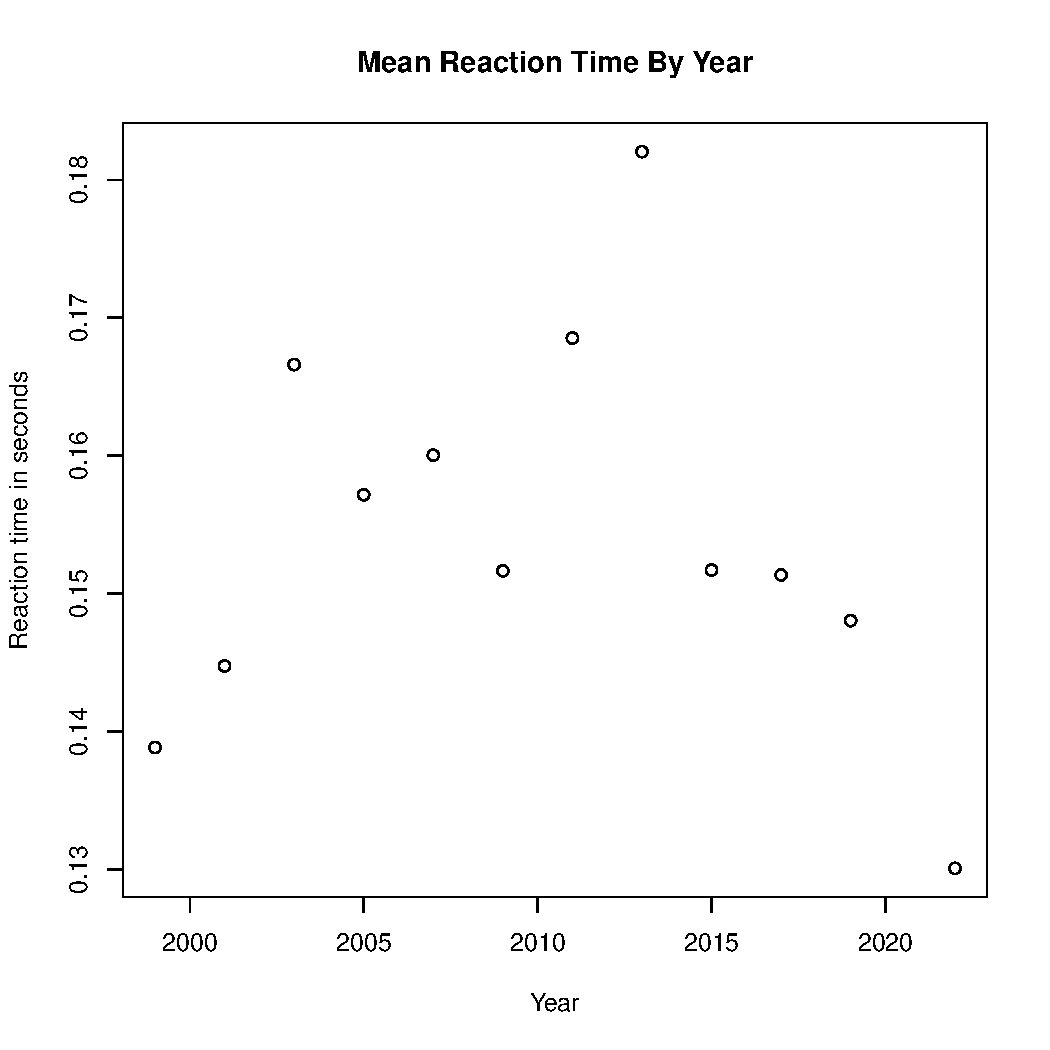
\includegraphics[scale = 0.6]{TBY}
  \label{fig:TBY}
\end{figure}

The figure below plots the average reaction time by year for the pooled men's data since
1999.  The circle in the bottom right is for 2022, which is signifcantly lower than the
data points for the previous three years, and is substially lower than the data points
for 2011 and 2013.  This graph supports the conclusion that the timing system from 2022
had some sort of error that caused the reaction times to be so much lower.  Assuming there
was not an issue with the system, the large variation is confusing because there is little explanation
as to why there is so much of a drop off in reaction time from 2013 to 2015 or the spike
from 2001 to 2003.

Devon Allen's disqulification at the World Track and Field Championships was
possibly the result of both a faulty timing equipment and Devon Allen
reacting extremely quickly to the start.  The code and data from R showed that
the 2022 World Track and Field Championships were a low outlier compared to
every other year in terms of average reaction time.  Addtionally, it was shown
through a gamma mixed effects model that there are significant year and batch
effects that greatly impact reaction time.  However, this practically does not make much sense
as there is no reason for so much random variation without much of a trend.
There has not been a consistent decrease or increase since 1999, much of the data
for reaction times has been random and unpredictable.  Thus while it seems easy
to conclude that Devon Allen was wrongly disqualified, that may not neccessarily
be the case.  If there are issues with reaction time such as athletes approaching the 0.10 
second barrier again at the next World Track Championship (August 2023), then World Athletics 
needs to adjust that threshold and allow for faster reaction times so that athletes with superb 
reflexes are not penalized like how Allen was in 2022.  World Athletics and Seiko 
may want to do further testing of their own to determine what is a human's physically
fastest reaction time, and if they choose to do so, they should start with Devon
Allen.


\section{Appendix}
\label{sec:appendix}
%Put downloadable data spreadsheet
Here is World Athletics website with the data: \url{https://www.worldathletics.org/results/world-athletics-championships}.
Here is the data for the USA Track and Field Championships: \url{https://www.flashresults.com/2022_Meets/Outdoor/06-23_USATF/}


\bibliographystyle{chicago}
\bibliography{citations.bib}


\end{document}
